\problemname{Karlsruhe Skyline}

\emph{Skyscrapers} is a grid logic puzzle in which numbers from $1$ to $n$ have to be placed into an $n\times n$ grid.
Each number needs to appear exactly once in each row and column.
These numbers are to be thought of as skyscrapers which are the respective number of units tall.
The rows and columns may have clue numbers on either end which describe the number of visible skyscrapers when looking down that row or column from that position, where taller buildings block the view of any shorter buildings behind them.

\begin{figure}[h]
	\centering
	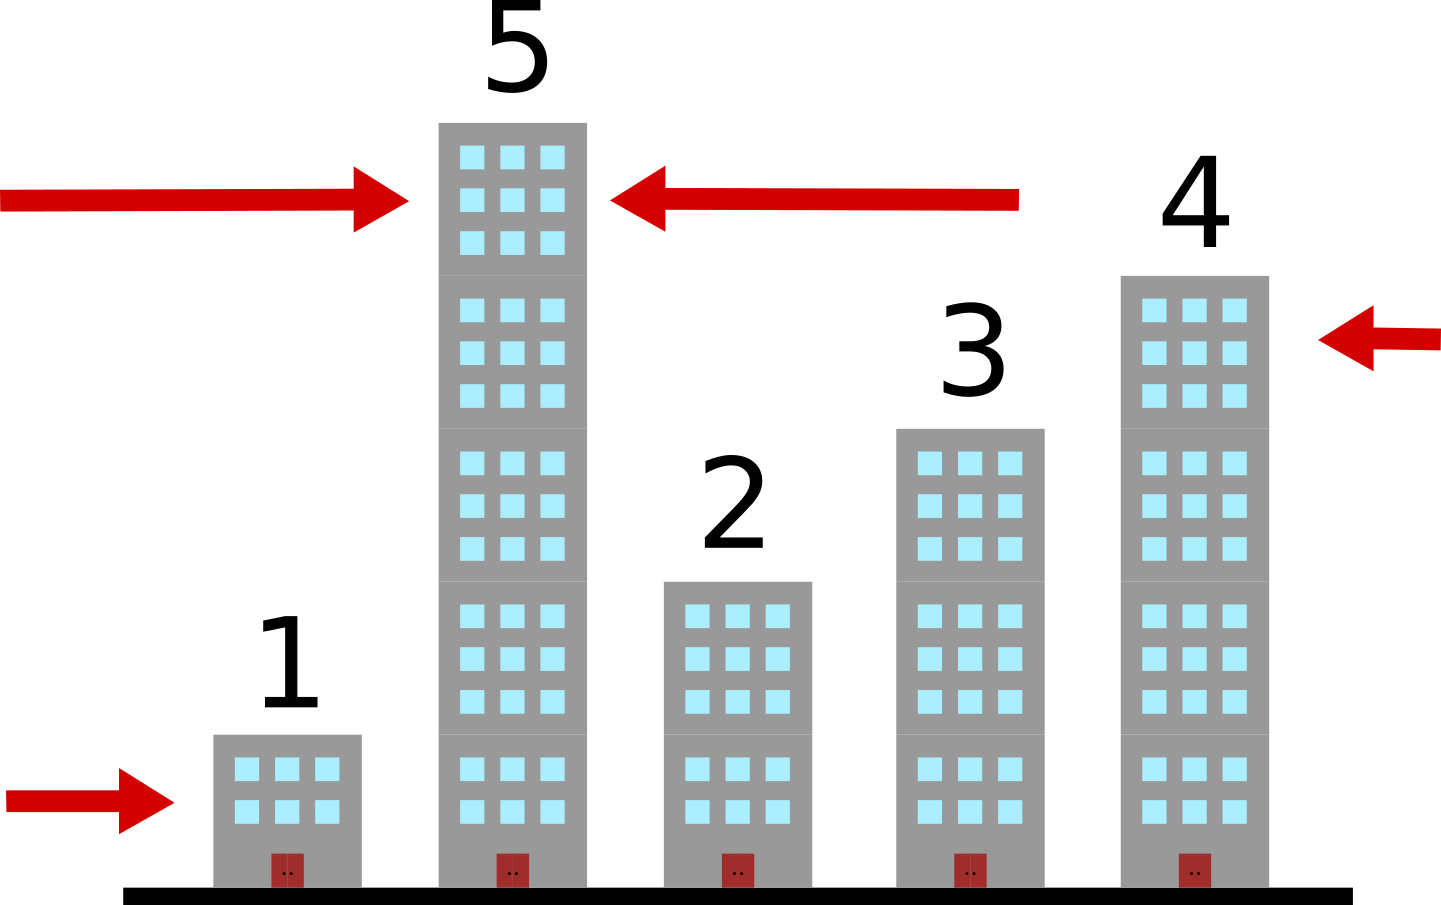
\includegraphics[width=0.5\textwidth]{sample1.png}
  \caption{Illustration of Sample Output 1. Two buildings (1 and 5) are visible from the left and two buildings (4 and 5) are visible from the right.}
\end{figure}

In this problem we consider only a single row of a Skyscrapers grid which has clue numbers on both ends.
Find out whether it is possible to place the skyscrapers from $1$ to $n$ in this row to satisfy both clues, and if so, find a valid placement.

\begin{Input}
  The input consists of:
  \begin{itemize}
    \item One line with three integers $n$, $a$ and $b$ ($2 \le n \le 1000$, $1 \le a,b \le n$), the length of the row and the clues on the left and right.
  \end{itemize}
\end{Input}

\begin{Output}
  If a valid placement exists, output ``\texttt{yes}'', followed by $n$ distinct integers $h_1,\dots,h_n$ ($1 \le h_i \le n$ for each $i$), the building heights from left to right.

  If there are multiple valid solutions, you may output any one of them.

  If no valid placement exists, output ``\texttt{no}''.
\end{Output}
